%----------------------------------------------------------------------------------------
% METADATA BLOCK (YAML)  — see inbox/README.md
%----------------------------------------------------------------------------------------
% uid: ""
% school: "lycee"
% level: "3eme"
% section: "Economie et Gestion"
% chapter: "Statistiques"
% title: "Quartiles d'une liste"
% difficulty: "Facile"
% tags: ["statistiques", "quartiles", "mediane", "diagramme-en-boite"]
% provenance: "own"
% batch: "2026-11-19-3eco-statistiques-n5"
%----------------------------------------------------------------------------------------

\newcommand{\R}{\mathbb{R}}
\newcommand{\vect}[1]{\overrightarrow{#1}}

% ---STATEMENT---
Voici l'âge des $15$ joueurs d'une équipe de handball :
\[22\quad19\quad30\quad17\quad25\quad21\quad33\quad19\quad24\quad28\quad18\quad22\quad26\quad20\quad23\]
\begin{enumerate}
  \item Ranger ces âges par ordre croissant, puis donner l'étendue.
  \item Déterminer la médiane, le premier quartile $Q_1$ et le troisième quartile $Q_3$. En déduire l'écart interquartile.
  \item Construire le diagramme en boîte de cette série.
  \item Quel pourcentage des joueurs a au moins $26$ ans ?
\end{enumerate}

% ---SOLUTION---
\begin{enumerate}[itemsep=14pt]
  \item Série rangée (rang au-dessus de chaque valeur) :
  \begin{center}\small
  \begin{tabular}{|*{15}{c|}}\hline
  $1$&$2$&$3$&$4$&$5$&$6$&$7$&$8$&$9$&$10$&$11$&$12$&$13$&$14$&$15$\\\hline
  $17$&$18$&$19$&$\mathbf{19}$&$20$&$21$&$22$&$\mathbf{22}$&$23$&$24$&$25$&$\mathbf{26}$&$28$&$30$&$33$\\\hline
  \end{tabular}\end{center}
  Étendue : $33-17=16$ ans.

  \item
  \begin{prop}[Médiane et quartiles (convention du manuel)]
  $n$ impair : la médiane est la valeur de rang \ib{$\dfrac{n+1}{2}$}.
  $Q_1$ est la valeur de rang $\dfrac n4$, $Q_3$ celle de rang $\dfrac{3n}{4}$ si ces nombres sont entiers ; sinon on prend \ib{le rang immédiatement supérieur}.
  \end{prop}
  $n=15$ : médiane de rang $8$ : $\text{Me}=22$.

  $\dfrac{15}{4}=3{,}75$, donc $Q_1$ est de rang $4$ : $Q_1=19$.

  $\dfrac{3\times15}{4}=11{,}25$, donc $Q_3$ est de rang $12$ : $Q_3=26$.
  \[\text{Écart interquartile : }Q_3-Q_1=26-19=7\text{ ans}\]

  \item
  \begin{center}
% alt: Diagramme en boîte : minimum 17, Q1 19, médiane 22, Q3 26, maximum 33.
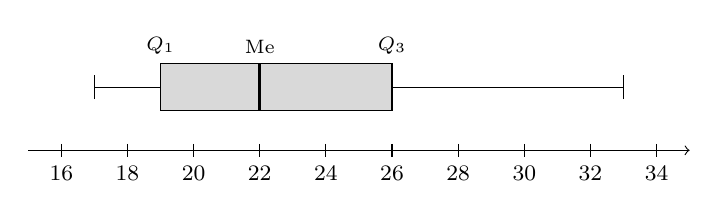
\begin{tikzpicture}[x=0.42cm,y=1cm]
    \draw[->] (15,0)--(35,0);
    \foreach \x in {16,18,...,34} {\draw (\x,0.08)--(\x,-0.08) node[below]{\footnotesize\x};}
    \draw (17,0.8)--(19,0.8); \draw (26,0.8)--(33,0.8);
    \draw[fill=gray!30] (19,0.5) rectangle (26,1.1); \draw[very thick] (22,0.5)--(22,1.1);
    \draw (17,0.65)--(17,0.95); \draw (33,0.65)--(33,0.95);
    \node[above,font=\scriptsize] at (19,1.1) {$Q_1$}; \node[above,font=\scriptsize] at (22,1.1) {Me}; \node[above,font=\scriptsize] at (26,1.1) {$Q_3$};
  \end{tikzpicture}
  \end{center}
  Boîte de $19$ à $26$, trait à $22$, moustaches de $17$ à $33$.

  \item Les joueurs d'au moins $26$ ans : $26$, $28$, $30$, $33$, soit $4$ joueurs sur $15$ :
  \[\dfrac{4}{15}\approx26{,}7\,\%\]
\end{enumerate}
